\section{Working with \rt transit data}
\label{sec:gtfs}

GTFS (general transit feed specification)
is an API (application programming interface) specification for transit data
detailing how it should be organised,
making access easier for application developers.
Developed and maintained by Google \citep{GoogleDevelopers_2006},
who make use of it in their Google Maps Transit Directions,
it is used by over 900~transit providers around the world,
including here in Auckland, New Zealand
(source \url{http://transitfeeds.com}).
An advantage of this standardised format is that,
provided an application depends solely on GTFS data,
after developing it locally in Auckland it can be deployed to any other GTFS-based
public transport system with minimal modification.


There are two components to GTFS.
The first, \emph{GTFS static}, includes information about
\begin{itemize}
\item \emph{stops}, a physical location where passengers can embark and disembark the vehicle;
\item \emph{routes}, a sequence of two or more stops displayed as a single service;
\item \emph{trips}, an instance of a route occuring at a specific time of day;
\item \emph{schedules}, specifying the arrival (and departure) times for each bus at each of its stops; 
\item \emph{shapes}, the sequence of points defining a vehicle's path along a route
\end{itemize}
\citep{GoogleDevelopers_2006}.
The second component is \emph{GTFS realtime},
which is only available in a subset of the providers due to the requirement of 
onboard GPS tracking devices and a central server.
It provides a standardised format for sharing vehicle positions and trip delays,
and are typically accessed by developers via an API can be used in \rt applications.

As mentioned in Section~\ref{sec:intro},
there are some major issues with the current ETA generation method.
These are almost directly attributed to GTFS-realtime trip updates,
which are currently the sole source of data for ETAs (in Auckland).
Trip updates are reported whenever a vehicle arrives or departs a stop,
and includes most importantly the delay between the scheduled and actual arrival times.
This delay is then propagated on to all future stops to adjust the ETA.
This assumes that the schedule is well calibrated and the time between scheduled arrivals
is representative of the real-world travel time between stops. 
Even more problematic is that, in the absense of trip updates,
the delay defaults to zero,
and unless the trip is manually cancelled,
appears on-time to passengers waiting at the stop.
If the bus is late or cancelled,
the trip disappears from the \rt board and passengers
are unable to distingush the two scenarios.


\subsection{Transit network construction}
\label{sec:network_build}

Arguably the most important predictor of arrival time is
the cumulative travel time along intermediate roads.
In most applications, however, this vital information is unavailable,
at least directly,
so here we attempt to construct a transit road network of intersections
and the roads between them, 
and map each route to a sequence of road segments.


The simplest way to construct such a network is to use the stop sequence:
routes with a common sub-sequence of stops must be traveling the same route between them,
so by defining a road as the path between two consecutive stops 
we can obtain travel time estimates along that road segment.
There are several places where this doesn't quite work, for example express routes 
and multi-stop locations where there are high numbers of routes,
resulting in some overlap between road segments,
it is a viable enough simplication for the purposes of this paper.
Figure~\ref{fig:network_creation} demonstrates how several overlapping routes 
are merged to form a road network.
In section~\ref{sec:kf} we present a model for estimating vehicle travel time
along a road segment.
Future work will look at using physical intersections as nodes in the network to improve it.

\begin{figure}[tb]
    \centering
    \begin{subfigure}{0.7\textwidth}
        \centering
        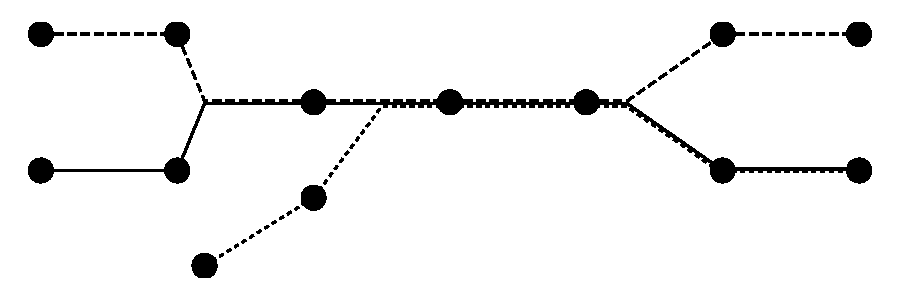
\includegraphics[width=0.95\textwidth]{figures/02_network_segments_1.pdf}
        \caption{Raw GTFS route shapes}
        \label{fig:network_creation_1}
    \end{subfigure} \\
    \begin{subfigure}{0.7\textwidth}
        \centering
        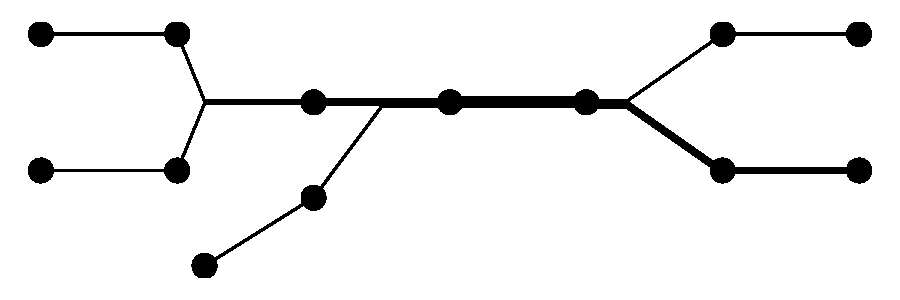
\includegraphics[width=0.95\textwidth]{figures/02_network_segments_2.pdf}
        \caption{GTFS-based road network}
        \label{fig:network_creation_2}
    \end{subfigure}
    \caption{Construction of a route network involves combining routes at nodes %
        (here we are using stops) which are connected by edges (roads). %
        In (a), the three unique routes, represented by different line types, clearly %
        overlap in several places. In (b) these have been merged, and the width of each line %
        represents how many routes use that link.}
    \label{fig:network_creation}
\end{figure}


\subsection{Realtime vehicle locations}
\label{sec:realtime_data}

GTFS \rt allows developers to query the current positions of vehicles
in the transit network.
The data consists of the time $t_k$ that the observation was made,
the GPS position of the vehicle, $\bY_k$, 
and some other information about the trip being serviced.
Vehicle positions are updated with a frequency of anywhere between 10~seconds and several minutes,
so there is often a lot of uncertainty about the trajectory
between two observations, particularly when there is one or more bus stop
or intersection between them.
It is also possible for a bus to remain stationary,
so the possible vehicle positions rapidly increases with the time between observations.


Another complication with the Auckland Transport realtime feed is that
the buses are programmed to report their location when arriving at
bus stops and some major intersections.
Often these updates are preemptive 
(i.e., the bus is almost there, but not quite),
and subsequent observations place the bus \emph{behind} the stop or intersection
(e.g., in a queue of traffic at traffic lights).
To handle this, we compute the approximate distance traveled, $\tilde x_k$,
of the vehicle by finding the nearest point on the path to the observation;
if this has decreased, the current state is rejected and the vehicle reverted
to its previous state.

